\documentclass[multi,preview,varwidth=false,border=5,12pt]{standalone}
%\documentclass[12pt]{article}

\newcounter{Qnum}
\usepackage{assignments}
\standaloneenv{question}


\excludecomment{solution}\let\endsolution\relax


\begin{document}


\begin{center}
\section*{Fluid Statics}
\end{center}




\begin{question}
The Mariana Trench is the deepest known point in the world's oceans. The maximum-known depth is about 36,000 ft.  Estimate the pressure at this depth assuming that the specific gravity of sea water is a constant of sg=1.03.  Report the result in psi.

\begin{solution}

\end{solution}

\end{question}


\begin{question}
If you dive without consciously equalizing the pressure in your ears it is possible to experience painful and damaging middle ear barotrauma.  At a pressure difference of about 15 kPa the tissue in the middle ear begins to tear and small blood vessels begin to expand and rupture resulting in inflammation and bruising which may take a few weeks to heal.  At what depth in meters would this start to occur if diving in fresh water?

\begin{solution}

\end{solution}

\end{question}


\begin{question}
A barometer indicates an atmospheric pressure of 30.12 inches of mercury.  Calculate the atmospheric pressure in mb (millibars).

\begin{solution}
$1020$ mb
\end{solution}

\end{question}

\begin{question}
The pressure in a heating duct is measured to be 4.16 in of H$_2$0.  What is this pressure in psi?

\begin{solution}
0.15 psi
\end{solution}

\end{question}


\begin{question}
The performance of a fan is rated at a pressure differential of 13.5 inWC. What is this pressure in Pa?

\begin{solution}
3360 Pa
\end{solution}

\end{question}

\begin{question}
A mercury manometer is used to measure the pressure at the bottom of a tank containing acetone.  What is the pressure in psig?  What is the depth, $d$, of the tank.

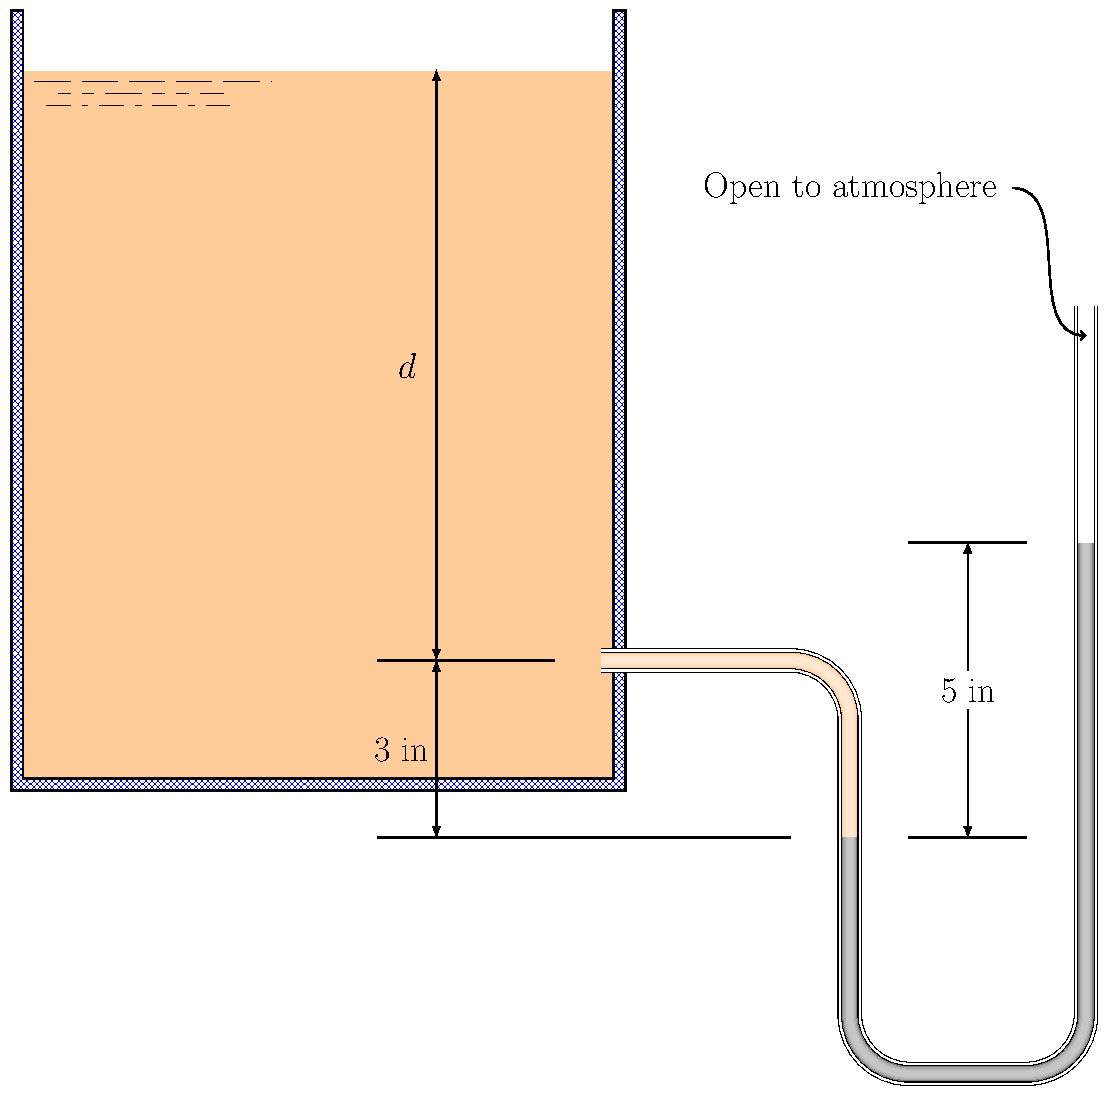
\includegraphics[width=4in]{imgs/mono1.pdf}


\begin{solution}
\end{solution}

\end{question}

\begin{question}
What is the pressure of the air in the tank for the system shown below.  Report your result in kPa (gauge).

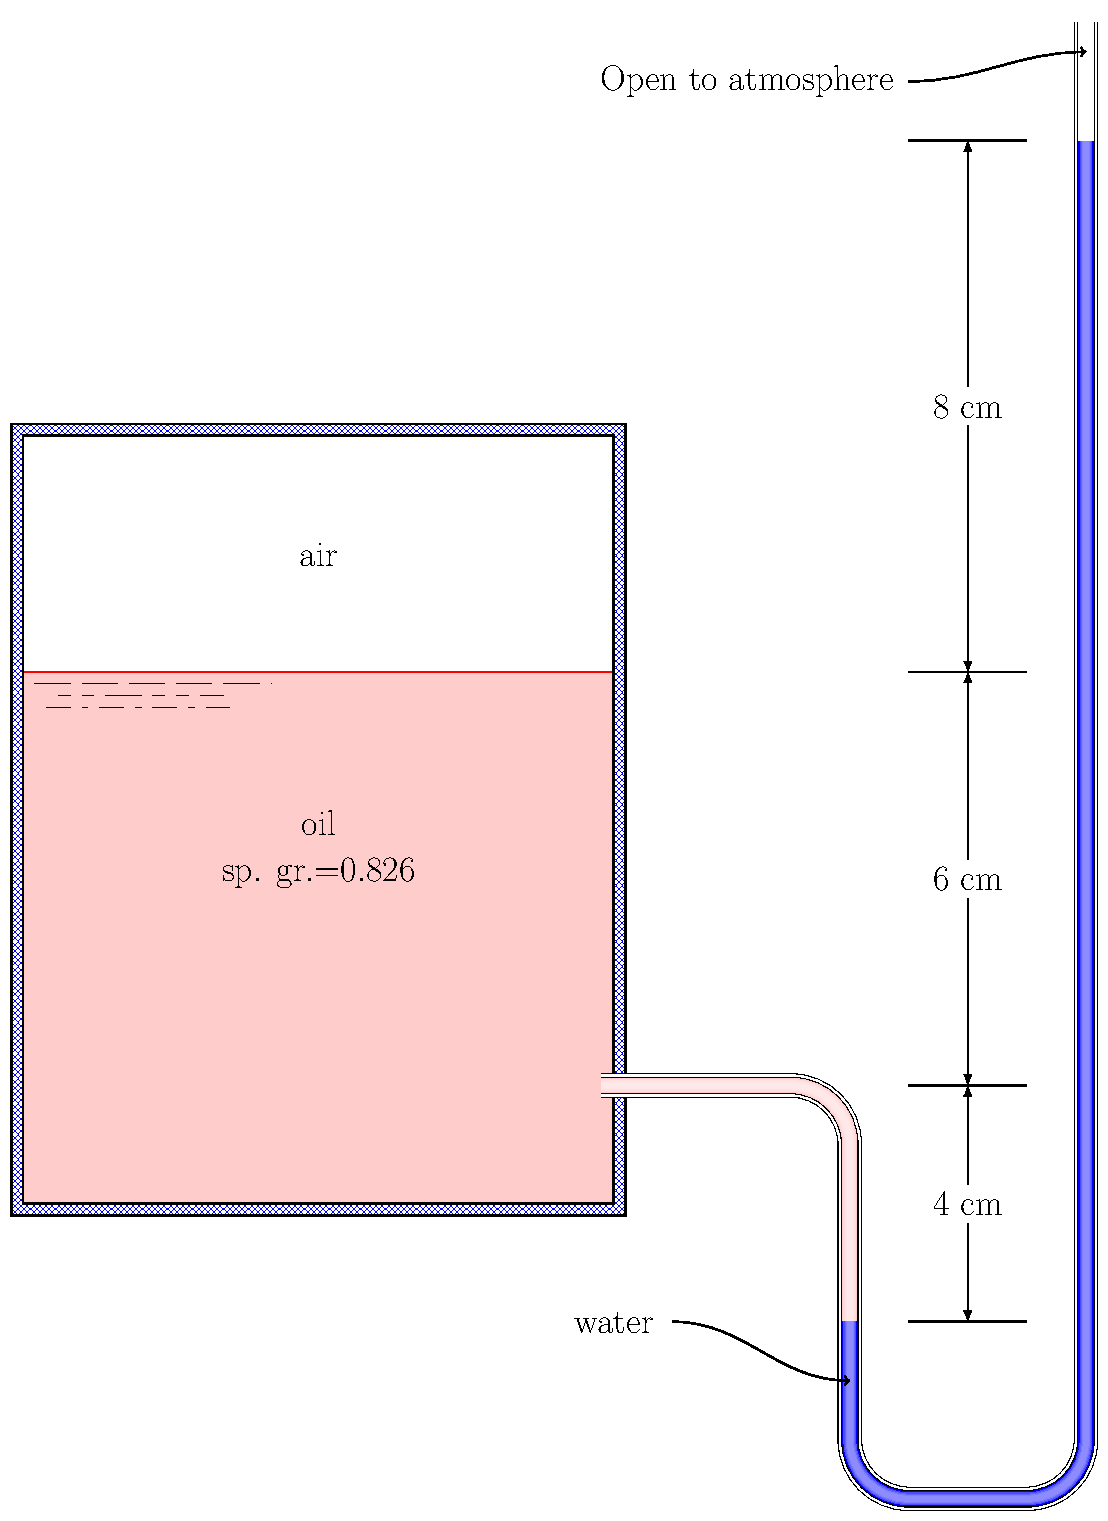
\includegraphics[width=4in]{imgs/mono2.pdf}


\begin{solution}
\end{solution}

\end{question}

\begin{question}
Calculate the pressure at point A in kPa (gauge).

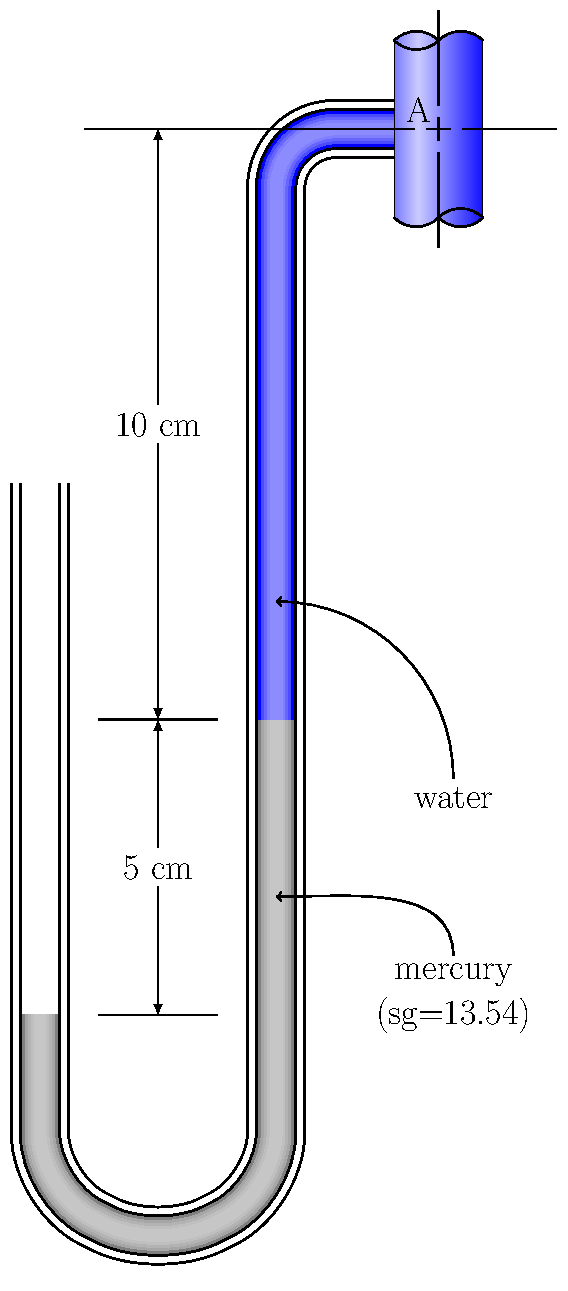
\includegraphics[width=2in]{imgs/mono3.pdf}


\begin{solution}
\end{solution}

\end{question}


\begin{question}
For the manometer shown in the figure below, calculate the quantity
$p_A - p_B$ in psi.  (Be sure to report the correct sign.)

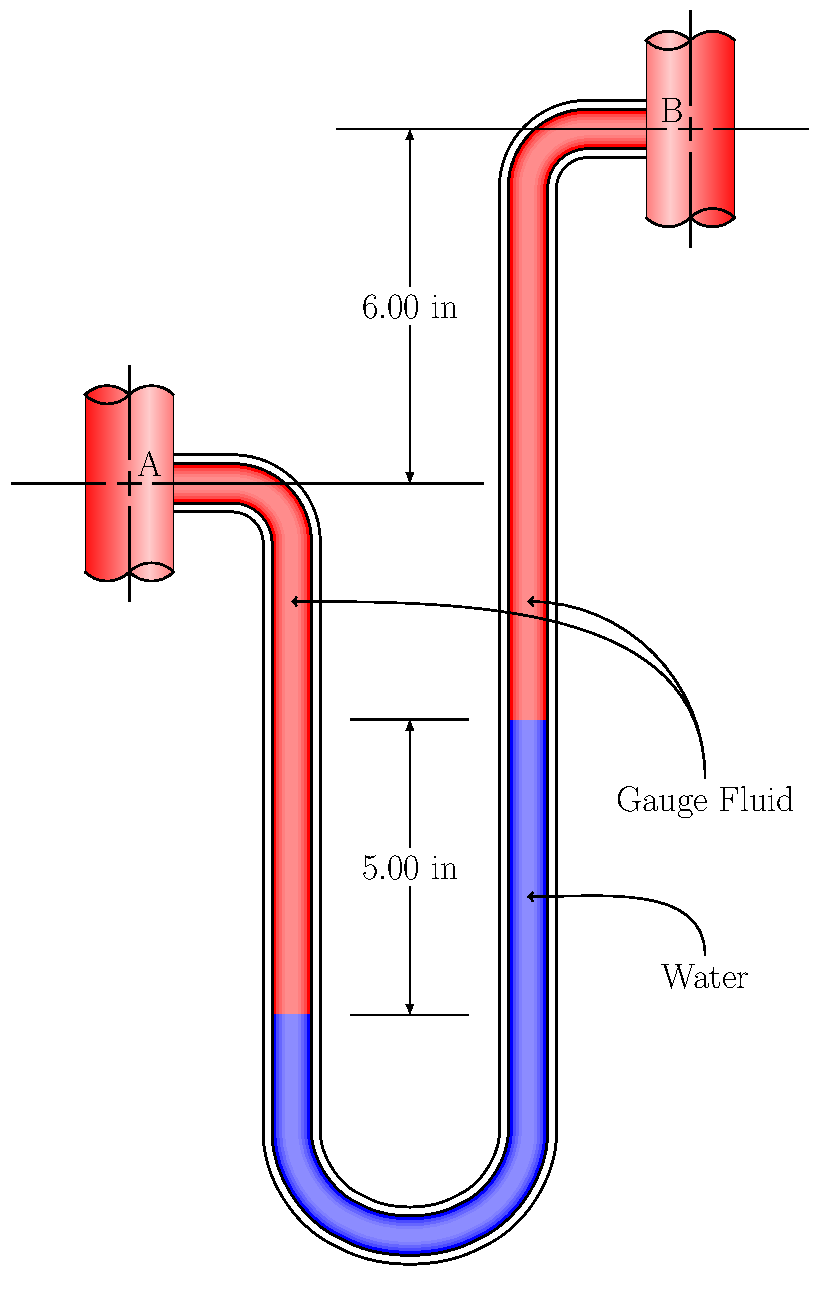
\includegraphics[width=3in]{imgs/mono4.pdf}


\begin{solution}
\end{solution}

\end{question}


\begin{question}

The following four problems concern the concrete
holding tank shown in figure 2. The tank is filled
with sludge (sg=1.4) to a height of 18 ft. The tank
is 40 ft long.

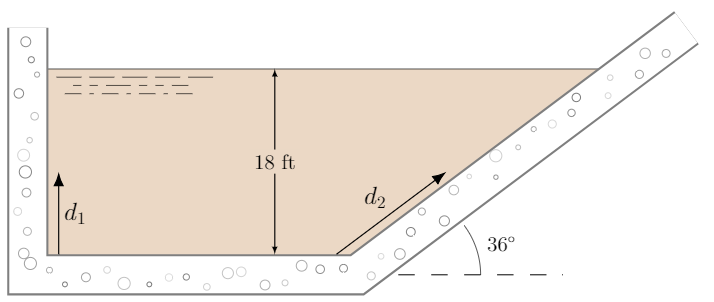
\includegraphics[width=4.5in]{imgs/SlurryWall.png}

What is the total force on the left wall?

\end{question}

\begin{question}
Determine the location of the center of pressure
($d_1$) on the left wall as measured from the
bottom of the tank.
\end{question}

\begin{question}
What is the total force on the right wall?
\end{question}

\begin{question}
Determine the location of the center of pressure
($d_2$) on the right wall as measured along the
face of the wall starting from the bottom of
the tank.
\end{question}


\begin{question}
Blood pressure is the pressure of circulating blood on the walls of large arteries and is usually expressed as the systolic pressure (maximum during one heart beat) over diastolic pressure (minimum in between beats).  In the U.S. it is measured in millimeters of mercury (mmHg), above the surrounding atmospheric pressure.  It is therefore a gauge pressure.

In Europe blood pressure is typically reported in kPa.  Convert a blood pressure reading of 135/90 mmHg into kPa.   Note that a blood pressure less than 120/80 mmHg is considered normal by the AHA.

\begin{solution}
18/12
\end{solution}

\end{question}

\begin{question}

Tonometry is a procedure to determine the fluid pressure inside the eye known as the intraocular pressure (IOP).  An elevated IOP is an important risk factor for glaucoma.  Applanation tonometry determines the IOP by by measuring the force required to flatten an area of the cornea.

If a 3.06~mm diameter probe flattens the corneal surface when a weight of 1.6 grams is applied, estimate the intraocular pressure in mmHg.  Note that a normal IOP is considered to be between 10 and 20 mmHg.

\begin{solution}
16
\end{solution}

\end{question}








\end{document}
